% ============================================================
%  Internal Report Draft
%  Component Counts, Hierarchy Proxies, and Merge-Tree Signals
%  in Wind-Field Super-Resolution
%
%  Format follows prior IEEEtran report/paper style.
%
%  Compile:
%    pdflatex main
%    bibtex main
%    pdflatex main
%    pdflatex main
% ============================================================
\documentclass[conference]{IEEEtran}

% --- Encoding and fonts ---
\usepackage[T1]{fontenc}
\usepackage[utf8]{inputenc}
\usepackage{times}
\usepackage{microtype}

% --- Math ---
\usepackage{amsmath}
\usepackage{amssymb}

% --- Citations ---
\usepackage{cite}

% --- Graphics and figures ---
\usepackage{graphicx}
\usepackage{subcaption}

% --- Tables ---
\usepackage{booktabs}
\usepackage{multirow}
\usepackage{array}
\usepackage{tabularx}

% --- Lists ---
\usepackage{enumitem}
\setlist[itemize]{noitemsep,topsep=2pt,leftmargin=*}

% --- Colors and hyperlinks ---
\usepackage{xcolor}
\usepackage{hyperref}
\hypersetup{colorlinks=true,citecolor=violet,linkcolor=blue,urlcolor=blue}

% --- Placeholder figure boxes ---
\newcommand{\placeholderfigure}[4]{%
\begin{figure*}[t]
    \centering
    \fbox{%
    \begin{minipage}[c][#4][c]{0.92\textwidth}
        \centering
        \textbf{#1}\\[0.5em]
        #2
    \end{minipage}}
    \caption{#3}
    \label{#1}
\end{figure*}}

\newcommand{\placeholderfigsingle}[4]{%
\begin{figure}[t]
    \centering
    \fbox{%
    \begin{minipage}[c][#4][c]{0.92\linewidth}
        \centering
        \textbf{#1}\\[0.5em]
        #2
    \end{minipage}}
    \caption{#3}
    \label{#1}
\end{figure}}

\newcommand{\methodwinner}[1]{\texttt{#1}}

\begin{document}

\title{Component Counts and Hierarchical Topology Proxies for Understanding Merge-Tree Behavior in Wind-Field Super-Resolution}

\author{%
\IEEEauthorblockN{Arjun Dadhwal}
\IEEEauthorblockA{Tulane University\\
Email: \texttt{[insert email]}}
}

\maketitle

\begin{abstract}
This report summarizes the component-count and topology-diagnostic stage of a wind-field super-resolution study. The broader project compares PhIRE-style CNN and GAN reconstructions, plus a non-learned bicubic/cubic interpolation baseline, on 168 consecutive hourly wind-field samples. Prior analysis showed a clear metric disagreement: direct-fidelity metrics such as PSNR, SSIM, speed error, and wind-power-density error strongly favor smooth outputs, while GAN outputs often perform better on distributional, spectral, gradient-distribution, and tail-sensitive measures. Persistence diagrams and merge trees also behave differently: persistence diagrams strongly favor GAN, whereas merge trees are more selective, choosing GAN in 20 of 168 samples. To make this merge-tree behavior more interpretable, this report introduces a superlevel-set connected-component analysis as a lightweight topology proxy. Across all samples, GAN is closest to ground truth in component count at lower thresholds ($t=5$ and $t=10$ m/s), while CNN becomes stronger at higher and percentile thresholds ($t=15$, p90, p95, p99). Bicubic interpolation is strong under direct-error metrics but severely under-represents component counts, indicating that it smooths away much of the topological complexity. The 20 MT-GAN cases separate into strong component-supported cases, low-threshold-only cases, and limitation cases. Adjacent temporal controls show that component counts do not fully explain MT decisions: in clusters such as 10--13 and 90--93, nearby samples have similar component signatures, but MT selects GAN for only one sample. This suggests that merge trees may encode hierarchical or nesting information beyond threshold-marginal component counts. The report closes by proposing additional merge-tree-relevant statistics, including component-count curves, branch persistence summaries, simplified-tree branch counts, and hierarchy proxies, as a bridge toward a topology-aware loss for scientific super-resolution.
\end{abstract}

\begin{IEEEkeywords}
Scientific visualization, wind-field super-resolution, component counts, merge trees, persistence diagrams, topology-aware learning, perception--distortion tradeoff.
\end{IEEEkeywords}

% ============================================================
\section{Motivation}
% ============================================================

The current project began as a post hoc evaluation of paired CNN and GAN outputs from a PhIRE-style wind-field super-resolution pipeline \cite{StengelPhIRE_2020}. The original goal was to study ambiguous cases where SSIM was close between the two models. After validating the fixed 168-sample evaluation set, however, SSIM selected CNN for every sample. This shifted the project from a near-tie analysis toward a broader question: what do different evaluators reward, and where do their preferences disagree?

The evaluation has now expanded to three reconstruction baselines:
\begin{itemize}
    \item \textbf{Bicubic/cubic interpolation}: a non-learned baseline that upsamples the $100\times100$ low-resolution vector input to $500\times500$.
    \item \textbf{CNN}: the smooth learned PhIRE baseline.
    \item \textbf{GAN}: the sharper learned PhIRE baseline.
\end{itemize}

A key finding is that the non-learned interpolation baseline is surprisingly strong on direct-fidelity metrics, while GAN remains stronger on several distributional and spectral metrics. This makes the evaluation problem sharper: good scientific SR should not merely be visually sharp, and it should not merely minimize point-wise error. Ideally, a future topology-aware model should retain bicubic/CNN-like direct accuracy while recovering more meaningful structural detail.

The merge-tree results provide the central motivation for the present report. Persistence diagrams select GAN in nearly all samples, whereas merge trees select GAN in only 20 of 168 samples. This suggests that topology is descriptor-specific: PD may reward GAN's additional persistent features, while MT may be more sensitive to whether those features fit the hierarchical organization of the ground truth scalar field.

The purpose of this report is to document the completed component-count and special-case analysis, then outline the next hierarchy-focused diagnostics needed before designing a topology-aware training objective.

% ============================================================
\section{Evaluation Setting}
% ============================================================

\placeholderfigure{fig:pipeline}{%
Replace with a schematic showing:
NREL WIND Toolkit $\rightarrow$ HR/GT vector fields $\rightarrow$ block-averaged MR input $\rightarrow$ bicubic/CNN/GAN reconstructions $\rightarrow$ scalar speed magnitude $\rightarrow$ direct metrics, physics/domain metrics, PD/MT, component counts, and hierarchy proxies.
}{%
Overview of the current evaluation pipeline. The report focuses on scalar wind-speed magnitude topology computed from vector-field outputs. The bicubic baseline provides a non-learned interpolation reference, while CNN and GAN provide smooth and sharp learned baselines, respectively.
}{1.55in}

\subsection{Scalar Representation}

All topological and component-count analyses are computed on scalar wind-speed magnitude,
\begin{equation}
    s(x,y) = \sqrt{u(x,y)^2 + v(x,y)^2},
\end{equation}
where $u$ and $v$ are the horizontal wind components. This scalarization follows the same representation used for the persistence-diagram and merge-tree comparisons.

\subsection{Metric Families}

The analysis combines several metric families:
\begin{itemize}
    \item \textbf{Direct fidelity}: PSNR, SSIM, speed MAE/RMSE, WPD MAE/RMSE, and gradient MAE.
    \item \textbf{Distributional/spectral structure}: WPD Wasserstein-1, PSD log-$L_2$, PSD slope error, gradient Wasserstein-1, and gradient-kurtosis error.
    \item \textbf{Tail behavior}: fixed-threshold and percentile-based exceedance-fraction errors.
    \item \textbf{Topology}: bottleneck persistence-diagram distance, merge-tree distance, and the connected-component proxies introduced here.
\end{itemize}

For signed quantities such as WPD bias, PSD slope difference, and gradient-kurtosis difference, the model with smaller absolute deviation from ground truth is treated as the winner.

% ============================================================
\section{All-Sample Baseline Results}
% ============================================================

\subsection{Selector Counts}

Table~\ref{tab:selector_counts} summarizes the key CNN/GAN selector counts from the post hoc topology stage. PSNR and SSIM favor CNN for all samples. PD heavily favors GAN. MT is selective, favoring GAN in 20 samples and CNN in 148.

\begin{table}[t]
\centering
\caption{CNN/GAN winner counts from the post hoc topology evaluation.}
\label{tab:selector_counts}
\begin{tabular}{lrrr}
\toprule
Selector / validator & CNN wins & GAN wins & Ties / unavailable \\
\midrule
$\mathrm{PSNR}_{uv}$ & 168 & 0 & 0 \\
SSIM & 168 & 0 & 0 \\
Bottleneck PD & 2 & 166 & 0 \\
Merge tree (MT) & 148 & 20 & 0 \\
Configured physics group & 168 & 0 & 0 \\
\bottomrule
\end{tabular}
\end{table}

\subsection{Three-Baseline Direct and Domain Metrics}

\begin{figure*}[t]
    \centering
    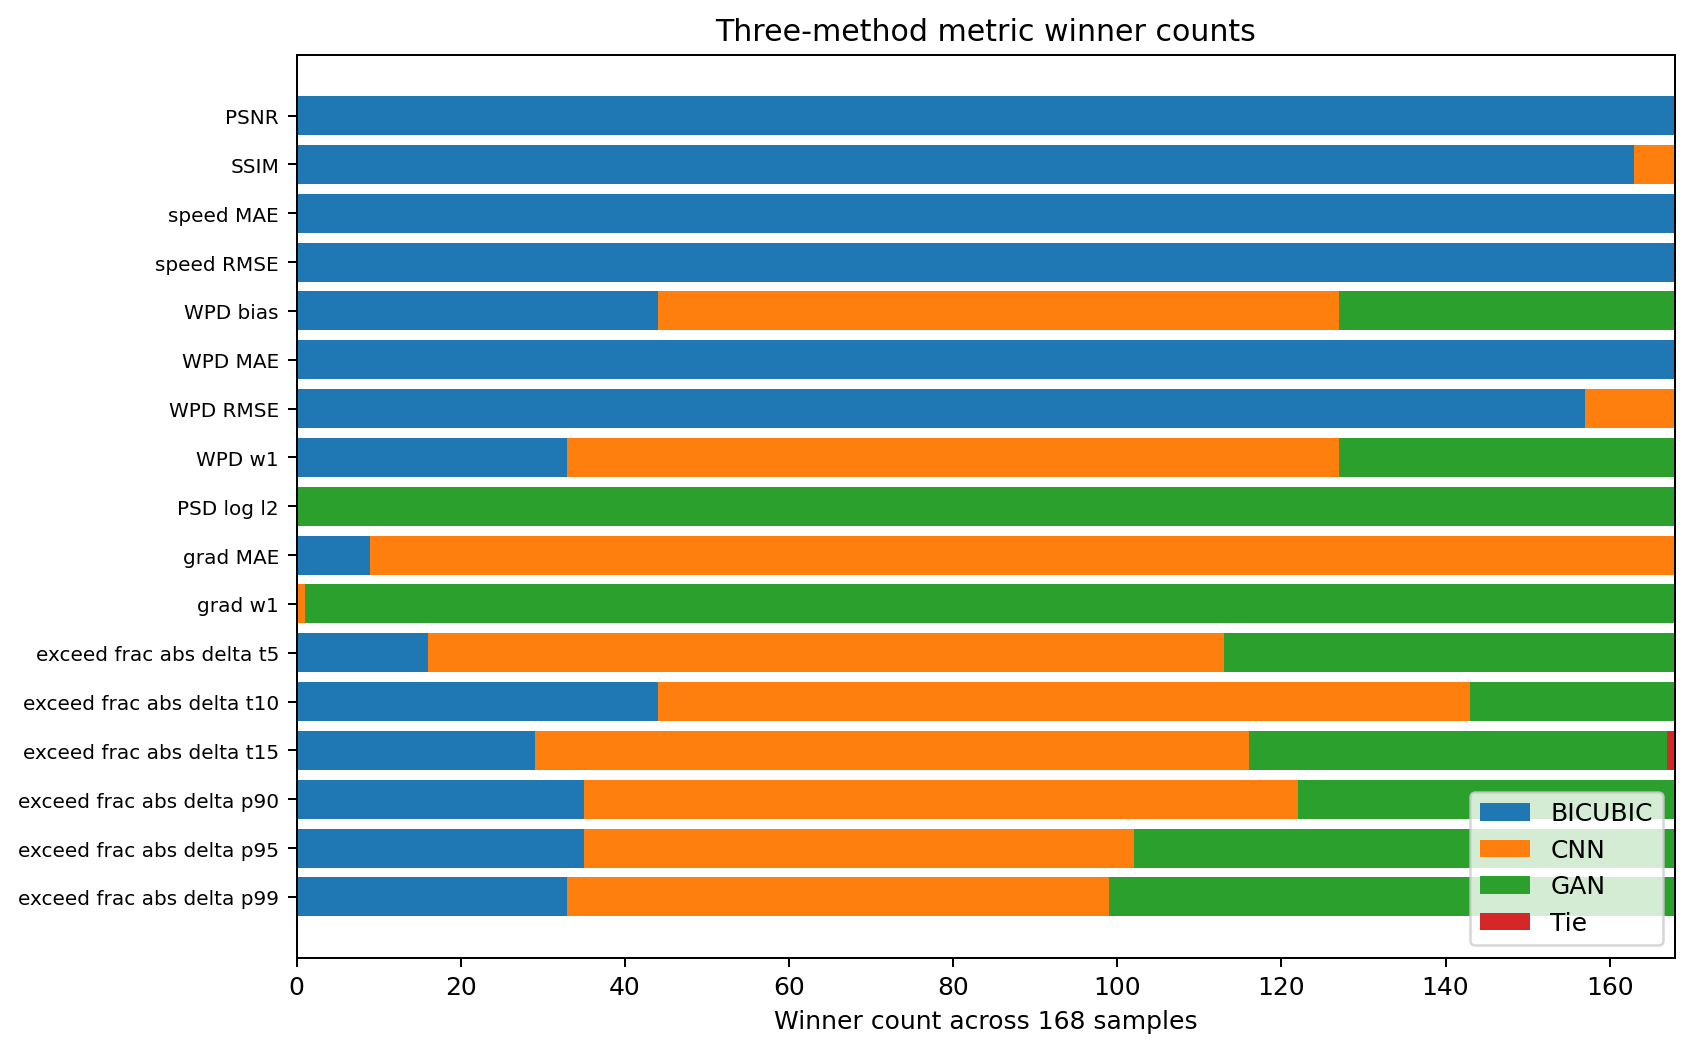
\includegraphics[width=0.95\textwidth]{figures/three_method_metric_summary.png}
    \caption{Three-method metric summary for bicubic, CNN, and GAN. Bicubic is expected to dominate many direct-fidelity metrics, while GAN remains stronger on several distributional and spectral metrics.}
    \label{fig:three_method_metric_summary}
\end{figure*}


The inclusion of bicubic/cubic interpolation changes the interpretation of the learned models. Bicubic is not merely a weak baseline: it is often the best direct-fidelity method. This suggests that the learned CNN/GAN outputs are not uniformly superior to classical interpolation on this evaluation slice. The future training objective should therefore be evaluated against bicubic as well as CNN and GAN.

% ============================================================
\section{Superlevel-Set Connected-Component Counts}
% ============================================================

\subsection{Definition}

To obtain an interpretable topology proxy, we count 8-connected components in superlevel sets of scalar wind-speed magnitude,
\begin{equation}
    C_{\tau}(s) = \# \mathrm{components}\{(x,y): s(x,y) \geq \tau\}.
\end{equation}
For each sample and each method, component counts are computed at six thresholds:
\begin{itemize}
    \item fixed physical thresholds: $t5$, $t10$, and $t15$ m/s;
    \item GT-relative percentile thresholds: p90, p95, and p99.
\end{itemize}
For each threshold, the winning method is the one whose component count is closest to the GT component count.

This proxy is intentionally simpler than a merge tree. It preserves the number of connected superlevel components at selected thresholds, but it discards how components are born, persist, nest, and merge across thresholds. Therefore, it is useful for interpretation but cannot fully explain MT behavior.

\subsection{Global Component-Count Summary}

Table~\ref{tab:component_summary} reports the all-sample component-count summary. The dominant pattern is threshold-dependent. GAN wins overwhelmingly at lower thresholds, especially $t5$ and $t10$, while CNN wins at higher and percentile thresholds. Bicubic almost always under-counts components.

\begin{table*}[t]
\centering
\caption{All-sample superlevel-set component-count summary. Winner counts indicate which method has component count closest to GT for each threshold.}
\label{tab:component_summary}
\begin{tabular}{lrrrrrrrr}
\toprule
Threshold & Mean GT & Mean $|err|$ Bicubic & Mean $|err|$ CNN & Mean $|err|$ GAN & Bicubic wins & CNN wins & GAN wins & Ties \\
\midrule
$t5$  & 91.6  & 79.29  & 64.38  & 23.82  & 1 & 30  & 134 & 3 \\
$t10$ & 336.6 & 271.81 & 187.17 & 72.89  & 0 & 17  & 150 & 1 \\
$t15$ & 213.1 & 177.58 & 116.81 & 149.91 & 0 & 99  & 68  & 1 \\
p90   & 286.6 & 232.78 & 149.28 & 223.58 & 4 & 104 & 59  & 1 \\
p95   & 220.6 & 181.34 & 113.00 & 182.88 & 0 & 111 & 57  & 0 \\
p99   & 113.0 & 96.64  & 62.86  & 94.52  & 2 & 103 & 63  & 0 \\
\bottomrule
\end{tabular}
\end{table*}

\begin{figure}[t]
    \centering
    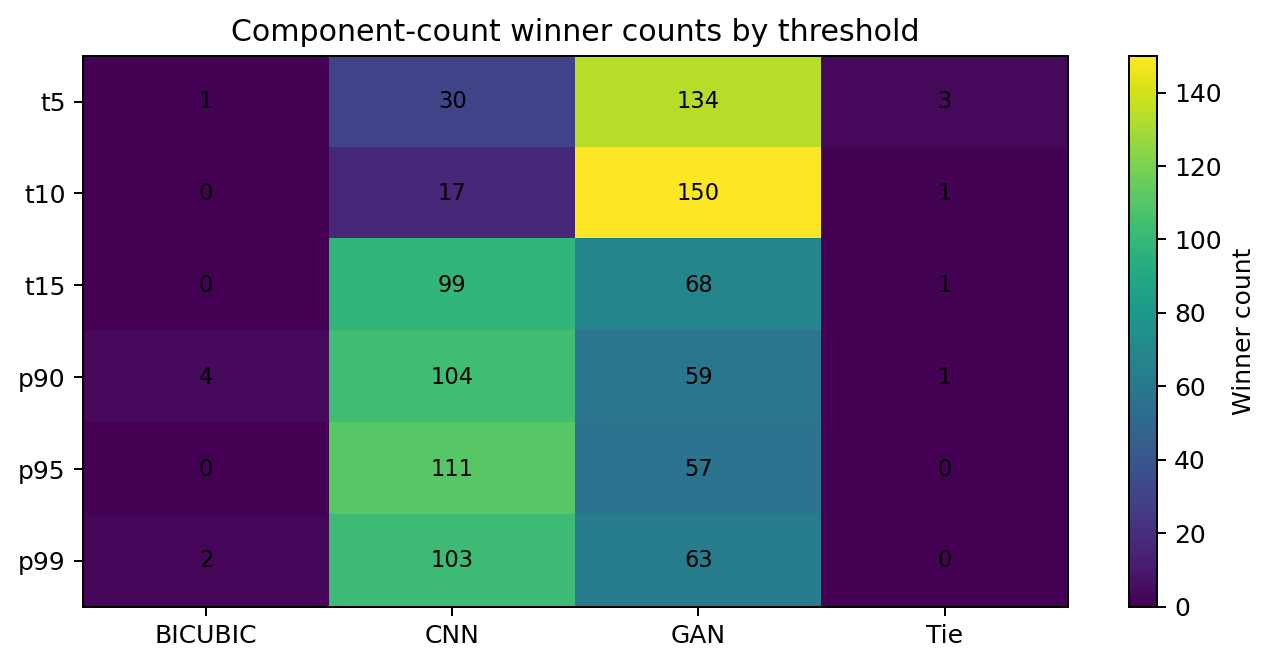
\includegraphics[width=\linewidth]{figures/component_threshold_heatmap.png}
    \caption{Component-count winner heatmap by threshold. GAN is closest to GT at lower thresholds, while CNN becomes stronger at higher and percentile thresholds.}
    \label{fig:component_threshold_heatmap}
\end{figure}



The global component-count result is important because it reconciles several earlier observations. GAN restores component complexity that bicubic and CNN often smooth away, especially at moderate thresholds. However, GAN also tends to over-fragment the high-speed tail, creating too many disconnected high-speed components at higher thresholds. CNN is smoother and often under-counts components, but its under-fragmentation can be less severe than GAN's over-fragmentation at high thresholds.

% ============================================================
\section{Special Case Analysis}
% ============================================================

\subsection{Case Families}

The special-case report organizes samples into five interpretive families:
\begin{itemize}
    \item \textbf{All MT-GAN cases}: the 20 samples where MT selects GAN.
    \item \textbf{Adjacent temporal clusters}: clusters 10--13, 76--78, and 90--93.
    \item \textbf{Rare topology-CNN cases}: samples 162 and 163, with neighbors 161 and 164.
    \item \textbf{Limitation cases}: samples 25, 80, and 154, where MT selects GAN but other evidence is weak or CNN-favoring.
    \item \textbf{GAN-majority but MT-CNN controls}: cases where GAN wins many domain metrics but MT rejects GAN.
\end{itemize}

The report is generated by \texttt{scripts/analyze\_special\_component\_cases.py} using the files under \texttt{ttk\_runs\_fixed/component\_counts/}.

\subsection{Threshold Signatures}

For each sample, we record a component-count winner signature:
\begin{equation}
    \sigma_i = [w_{t5}, w_{t10}, w_{t15}, w_{p90}, w_{p95}, w_{p99}],
\end{equation}
where $w_{\tau}\in\{\mathrm{Bicubic},\mathrm{CNN},\mathrm{GAN},\mathrm{Tie}\}$ is the method with component count closest to GT at threshold $\tau$.

\begin{figure}[t]
    \centering
    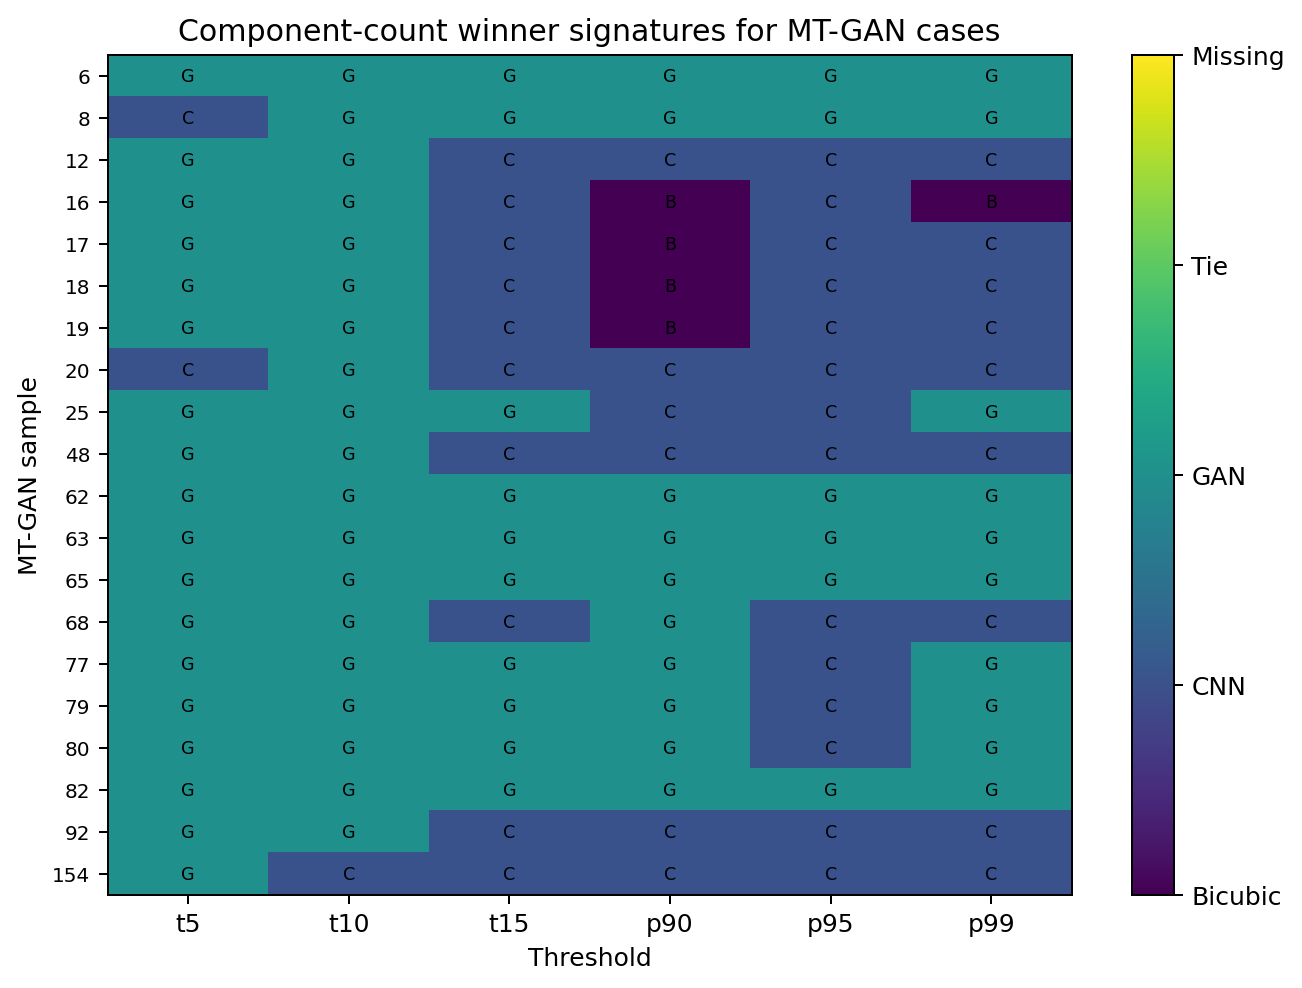
\includegraphics[width=\linewidth]{figures/mt_gan_signature_matrix.png}
    \caption{Component-count winner signatures for the 20 MT-GAN cases. Rows are samples and columns are thresholds. This separates strong GAN-supported cases from low-threshold-only and limitation cases.}
    \label{fig:mt_gan_signature_matrix}
\end{figure}


The 20 MT-GAN cases are heterogeneous. Some show strong component-count support for GAN across thresholds, while many support GAN only at low thresholds. This heterogeneity is important: MT-GAN does not mean ``GAN is better everywhere.'' Instead, MT-GAN marks a structural-disagreement subset that requires deeper analysis.

\subsection{Interpretation Labels}

The special-case report assigns one of five interpretation labels:
\begin{itemize}
    \item \textbf{GAN\_component\_strong}: GAN wins at least four of six thresholds.
    \item \textbf{GAN\_component\_low\_threshold\_only}: GAN wins mainly at $t5$ and $t10$.
    \item \textbf{GAN\_component\_overfragmented\_high\_threshold}: GAN over-fragments high-speed components relative to GT.
    \item \textbf{CNN\_component\_control}: CNN wins at least four of six thresholds.
    \item \textbf{mixed\_or\_ambiguous}: no clear method dominates.
\end{itemize}

For the curated cases, the observed label distribution is shown in Table~\ref{tab:curated_label_distribution}.

\begin{table}[t]
\centering
\caption{Interpretation-label distribution among curated special cases.}
\label{tab:curated_label_distribution}
\begin{tabular}{lr}
\toprule
Interpretation label & Count \\
\midrule
GAN component low-threshold only & 16 \\
GAN component strong & 5 \\
GAN over-fragmented at high threshold & 1 \\
Mixed or ambiguous & 1 \\
\bottomrule
\end{tabular}
\end{table}

% ============================================================
\section{Adjacent Temporal Controls}
% ============================================================

Adjacent temporal controls are especially valuable because neighboring sample IDs correspond to neighboring timesteps. They provide local controls for atmospheric regime, spatial domain, and temporal context.

\begin{figure*}[t]
    \centering
    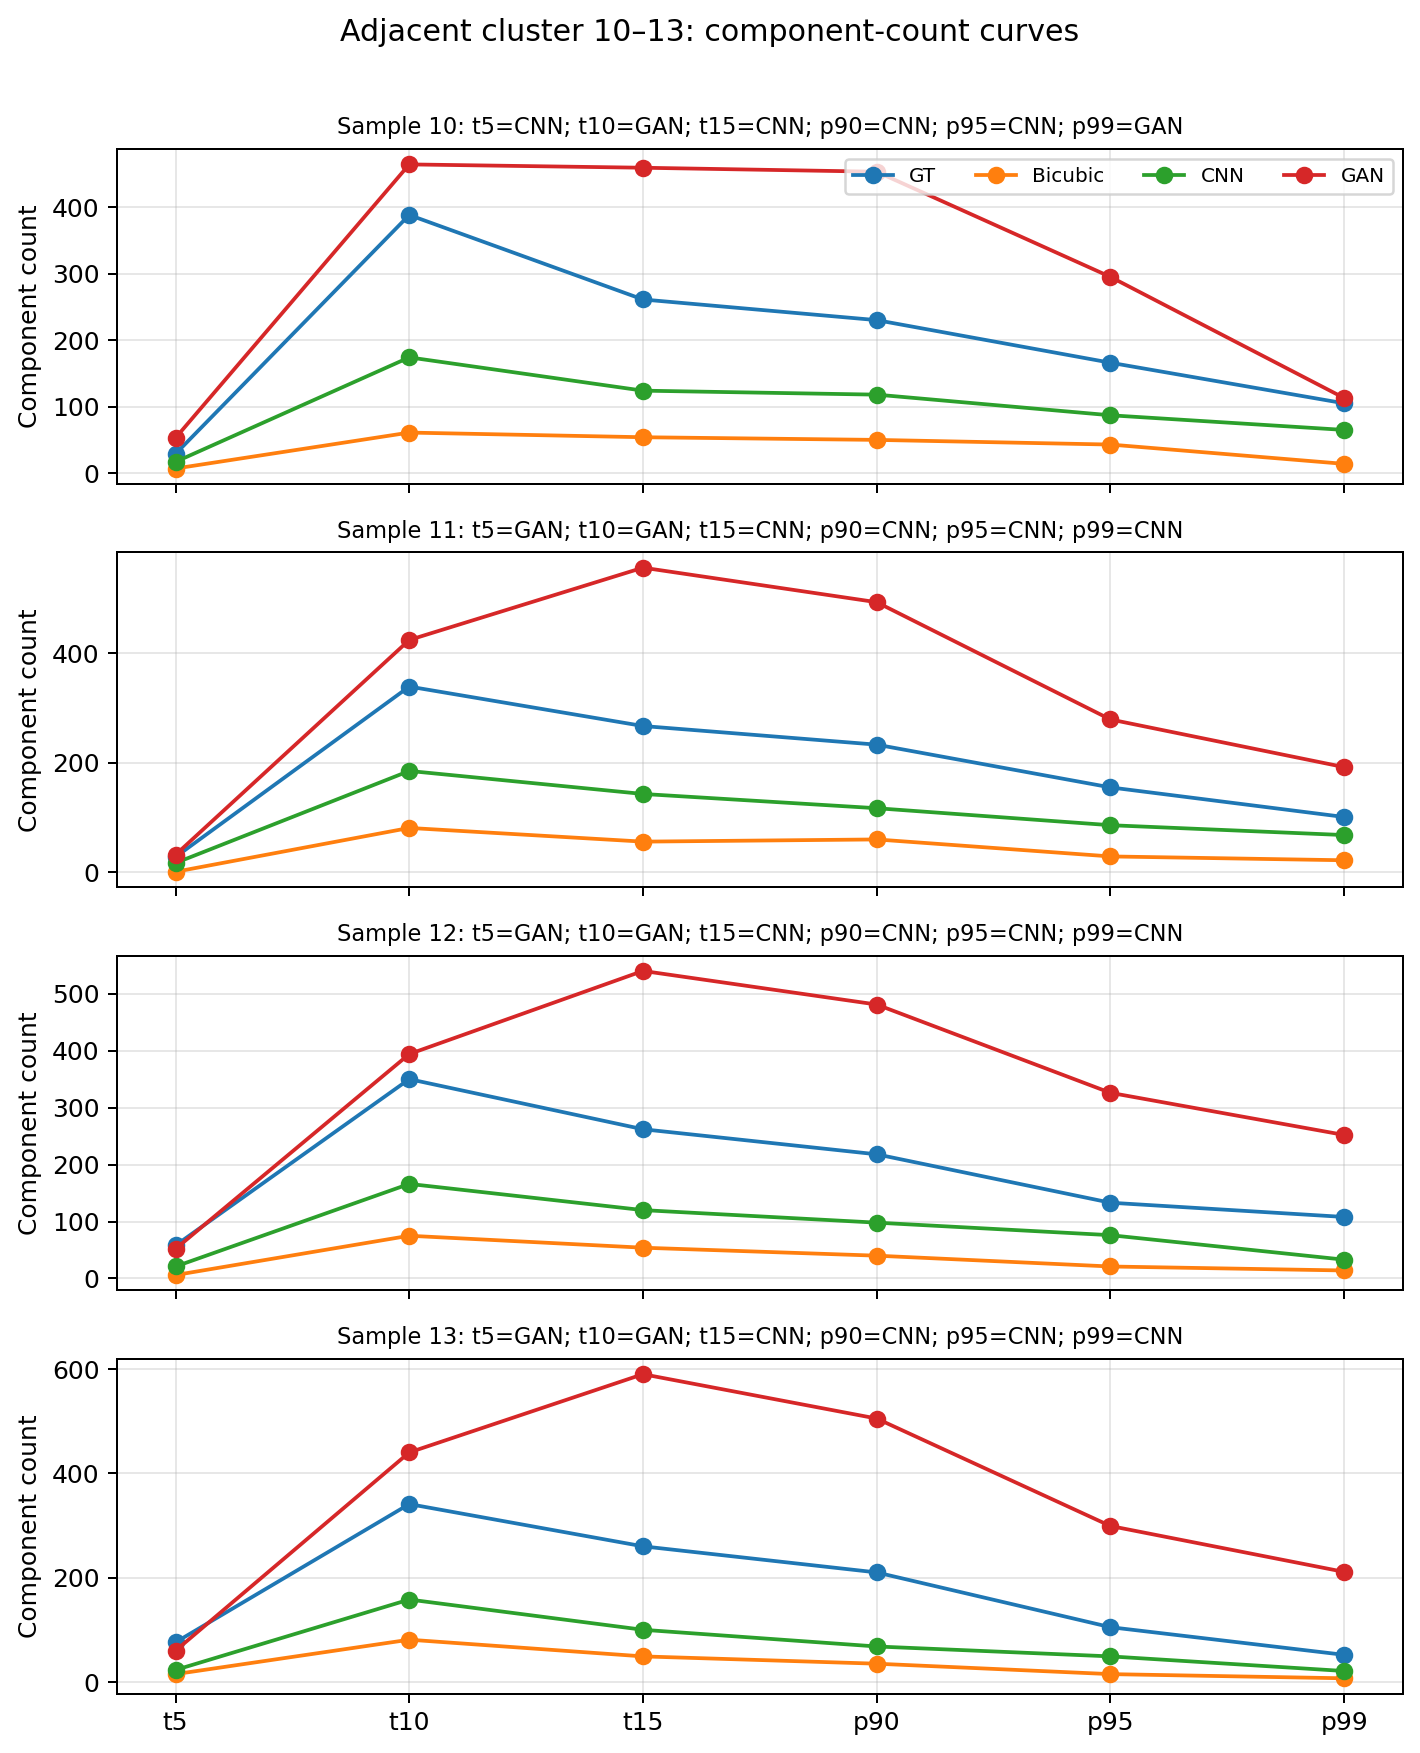
\includegraphics[width=0.92\textwidth]{figures/adjacent_component_curves_10_13.png}
    \caption{Component-count curves for adjacent cluster 10--13. Sample 12 is MT-GAN, while neighboring samples are MT-CNN. Similar curves with different MT decisions suggest that simple component counts do not fully explain MT behavior.}
    \label{fig:adjacent_component_curves_10_13}
\end{figure*}

\begin{figure*}[t]
    \centering
    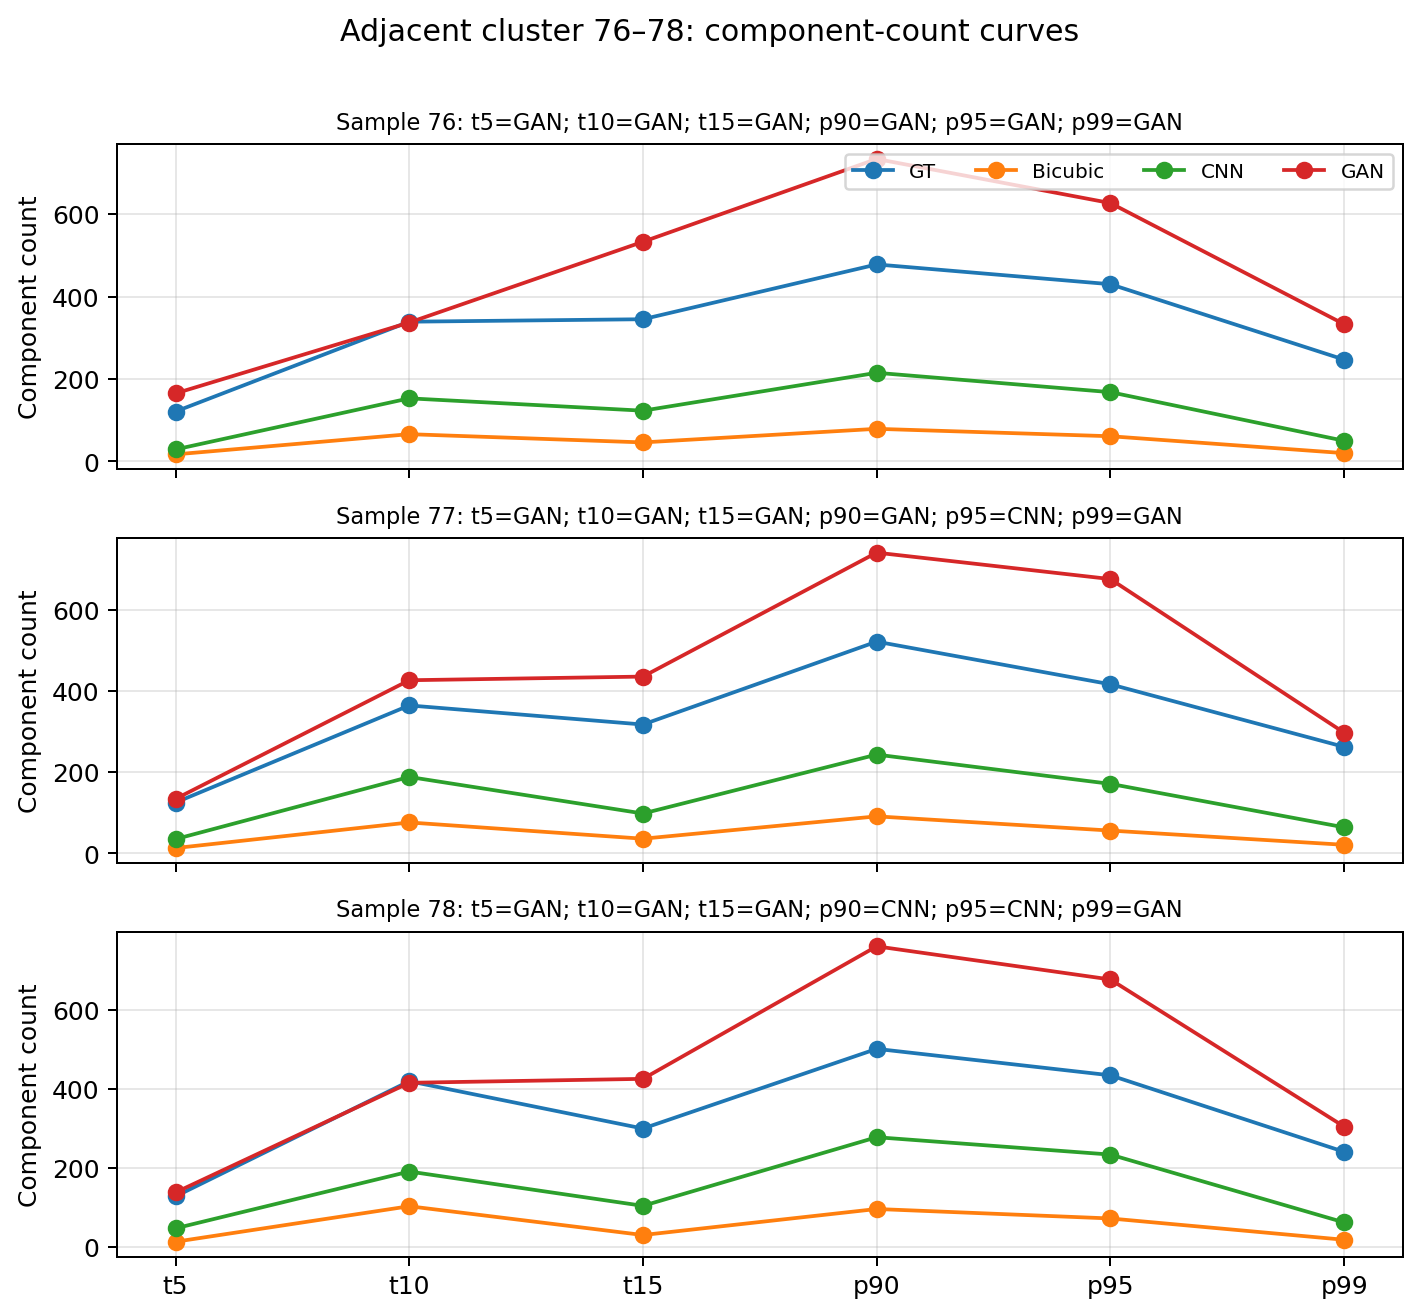
\includegraphics[width=0.92\textwidth]{figures/adjacent_component_curves_76_78.png}
    \caption{Component-count curves for adjacent cluster 76--78. This cluster tests whether sample 77's MT-GAN selection has a distinct component-count signature relative to neighboring timesteps.}
    \label{fig:adjacent_component_curves_76_78}
\end{figure*}

\begin{figure*}[t]
    \centering
    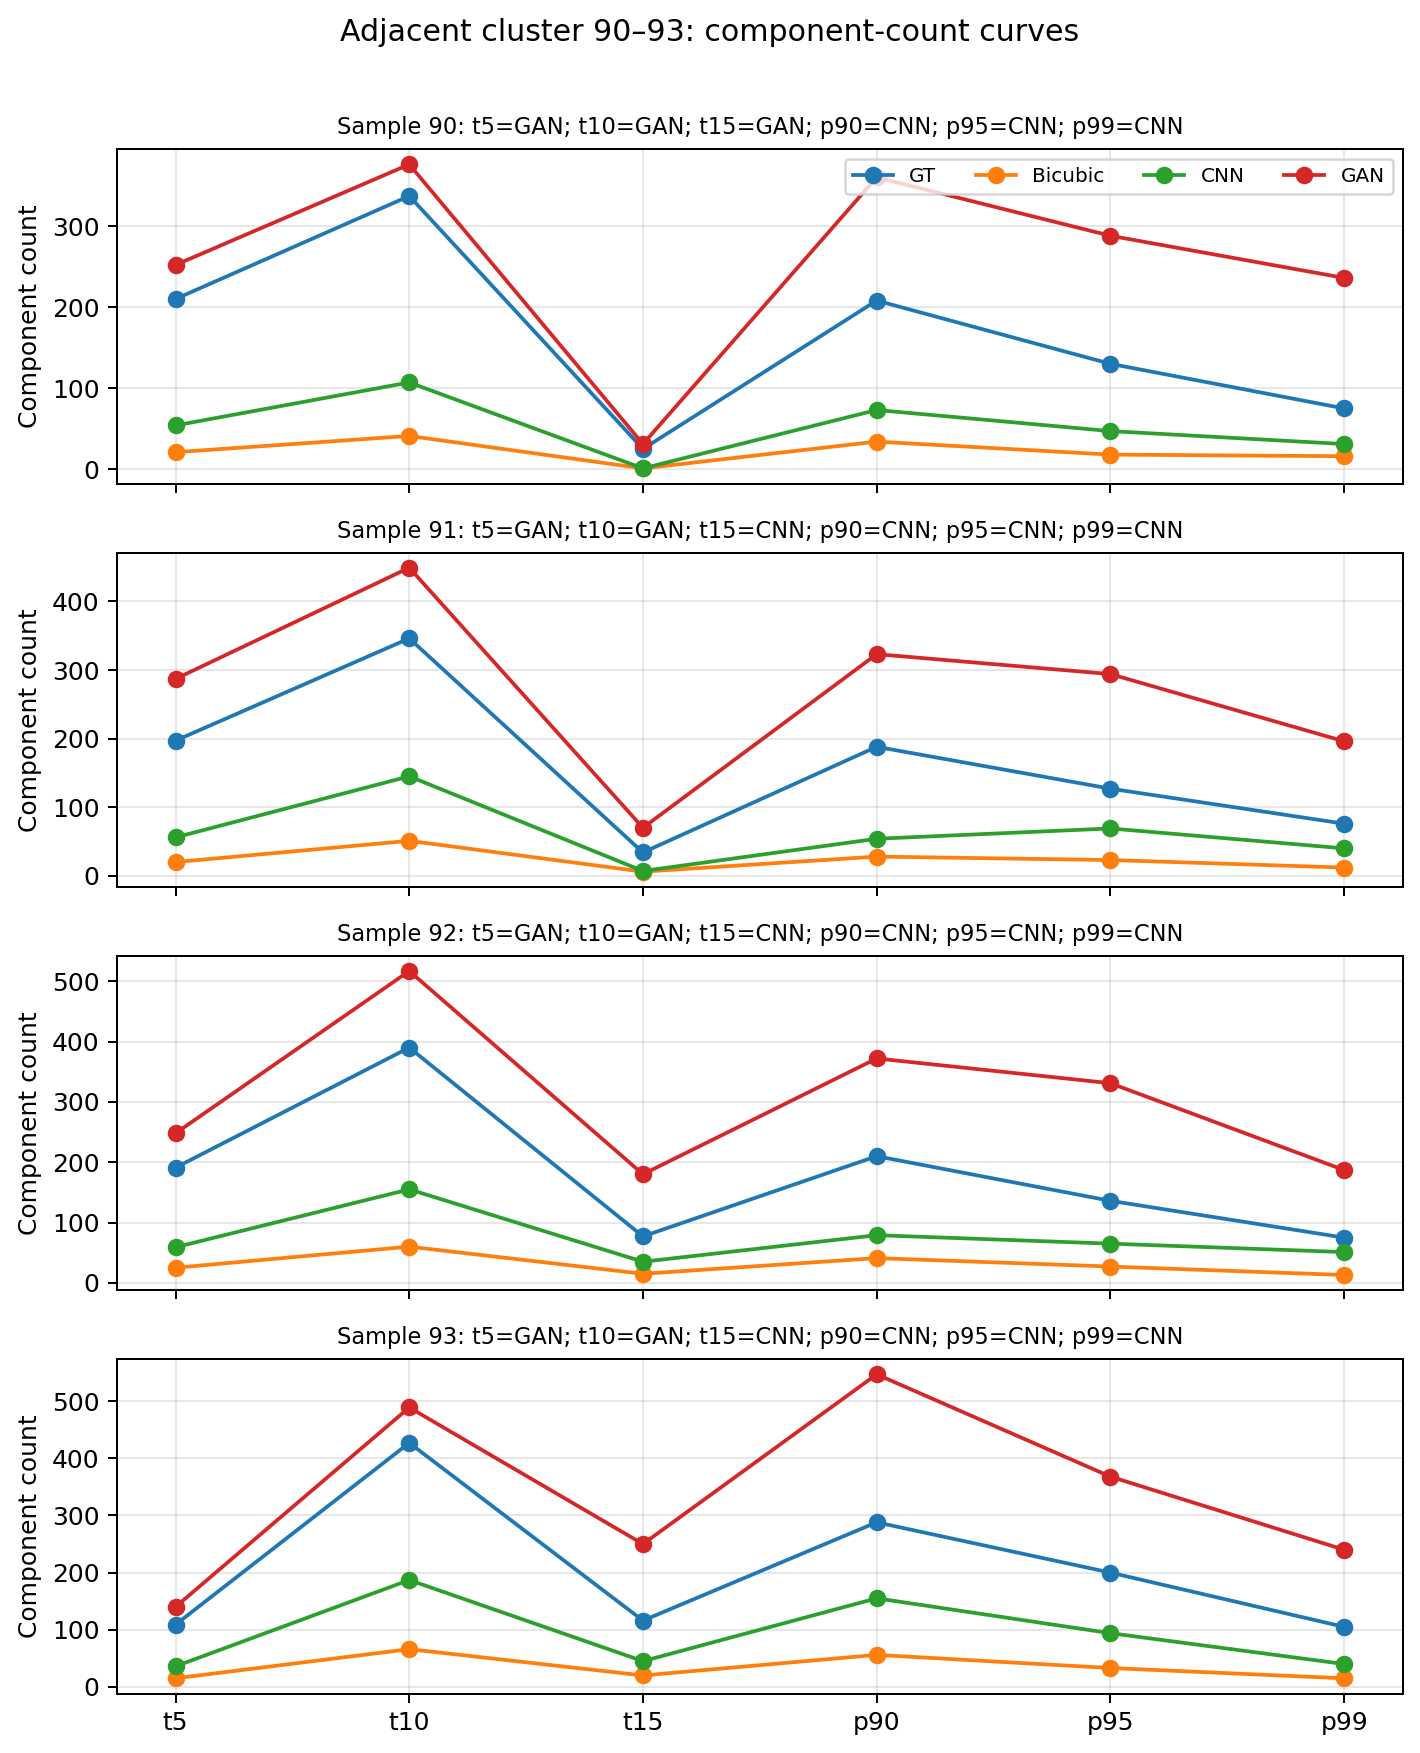
\includegraphics[width=0.92\textwidth]{figures/adjacent_component_curves_90_93.png}
    \caption{Component-count curves for adjacent cluster 90--93. Sample 92 is MT-GAN, while nearby GAN-majority samples remain MT-CNN.}
    \label{fig:adjacent_component_curves_90_93}
\end{figure*}


In clusters such as 10--13 and 90--93, the component signatures can remain similar while MT flips only for a single sample. This is a central interpretive result. If simple component counts cannot distinguish the MT-GAN sample from its neighbors, then MT is likely sensitive to information that component counts discard: the hierarchy of how components are nested, born, and merged across thresholds.

% ============================================================
\section{Rare Topology-CNN Controls}
% ============================================================

\begin{figure*}[t]
    \centering
    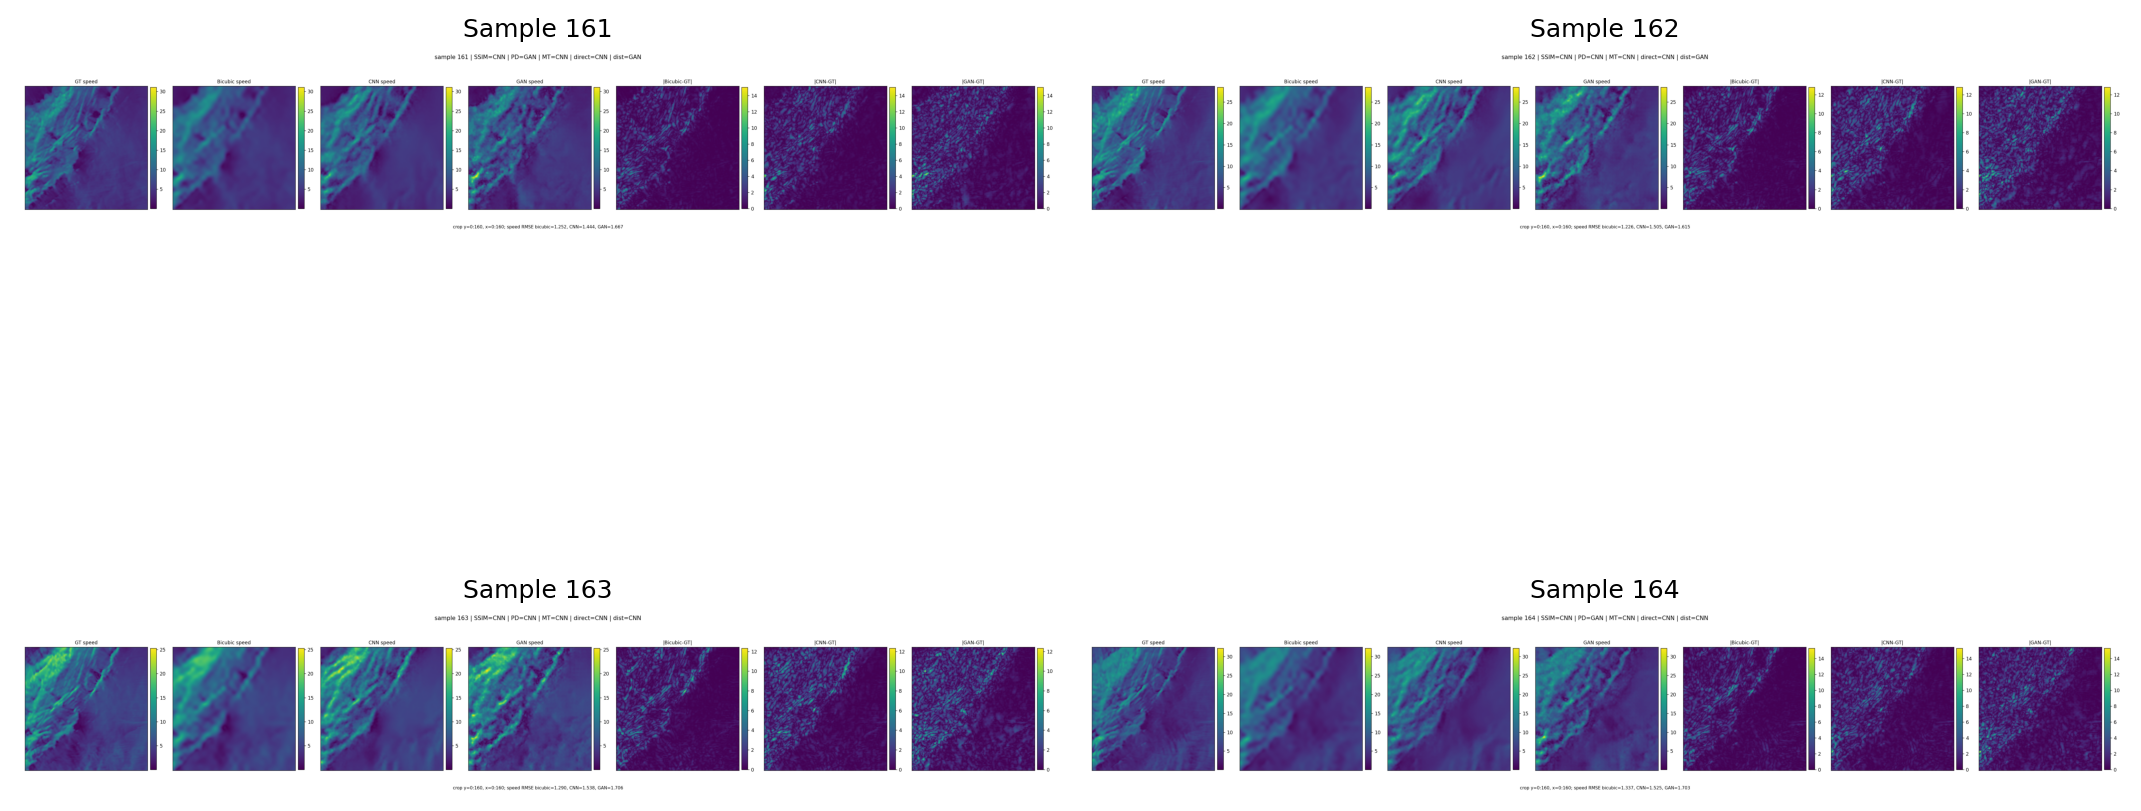
\includegraphics[width=0.92\textwidth]{figures/topology_cnn_controls.png}
    \caption{Rare topology-CNN controls. Samples 162 and 163 are important because both PD and MT select CNN, showing that topology does not automatically favor GAN.}
    \label{fig:topology_cnn_controls}
\end{figure*}

The rare PD=MT=CNN samples are important negative controls. PD normally favors GAN, but in these cases even PD selects CNN. This suggests that the GAN-generated structures are not only sharp but also topologically inconsistent under both descriptor families. These samples should be inspected with both visual panels and component/hierarchy summaries.

% ============================================================
\section{Toward Hierarchical Merge-Tree Proxies}
% ============================================================

The current component-count analysis is only a first-order proxy. It records how many connected components exist at selected thresholds, but it does not describe how those components relate across thresholds. Merge trees, by contrast, encode a hierarchy: which components appear, persist, nest, and merge as the threshold changes \cite{Yan_2021,YanDissertation_2022}. The next stage should therefore add hierarchy-aware statistics that are still easier than full MT visualization.

\subsection{Dense Component-Count Curves}

Instead of six thresholds, compute component counts across $K=30$--$50$ thresholds. For each method, define the component-count curve:
\begin{equation}
    \beta_0^{m}(\tau_k) = C_{\tau_k}(s_m), \quad k=1,\dots,K.
\end{equation}
Then compare each SR method to GT using:
\begin{equation}
    E_{\beta_0}^{m} = \sum_{k=1}^{K} \left|\beta_0^{m}(\tau_k) - \beta_0^{GT}(\tau_k)\right|.
\end{equation}
This gives a richer version of the current component-count proxy and may reveal where MT-GAN samples diverge from adjacent controls.

\begin{figure*}[t]
    \centering
    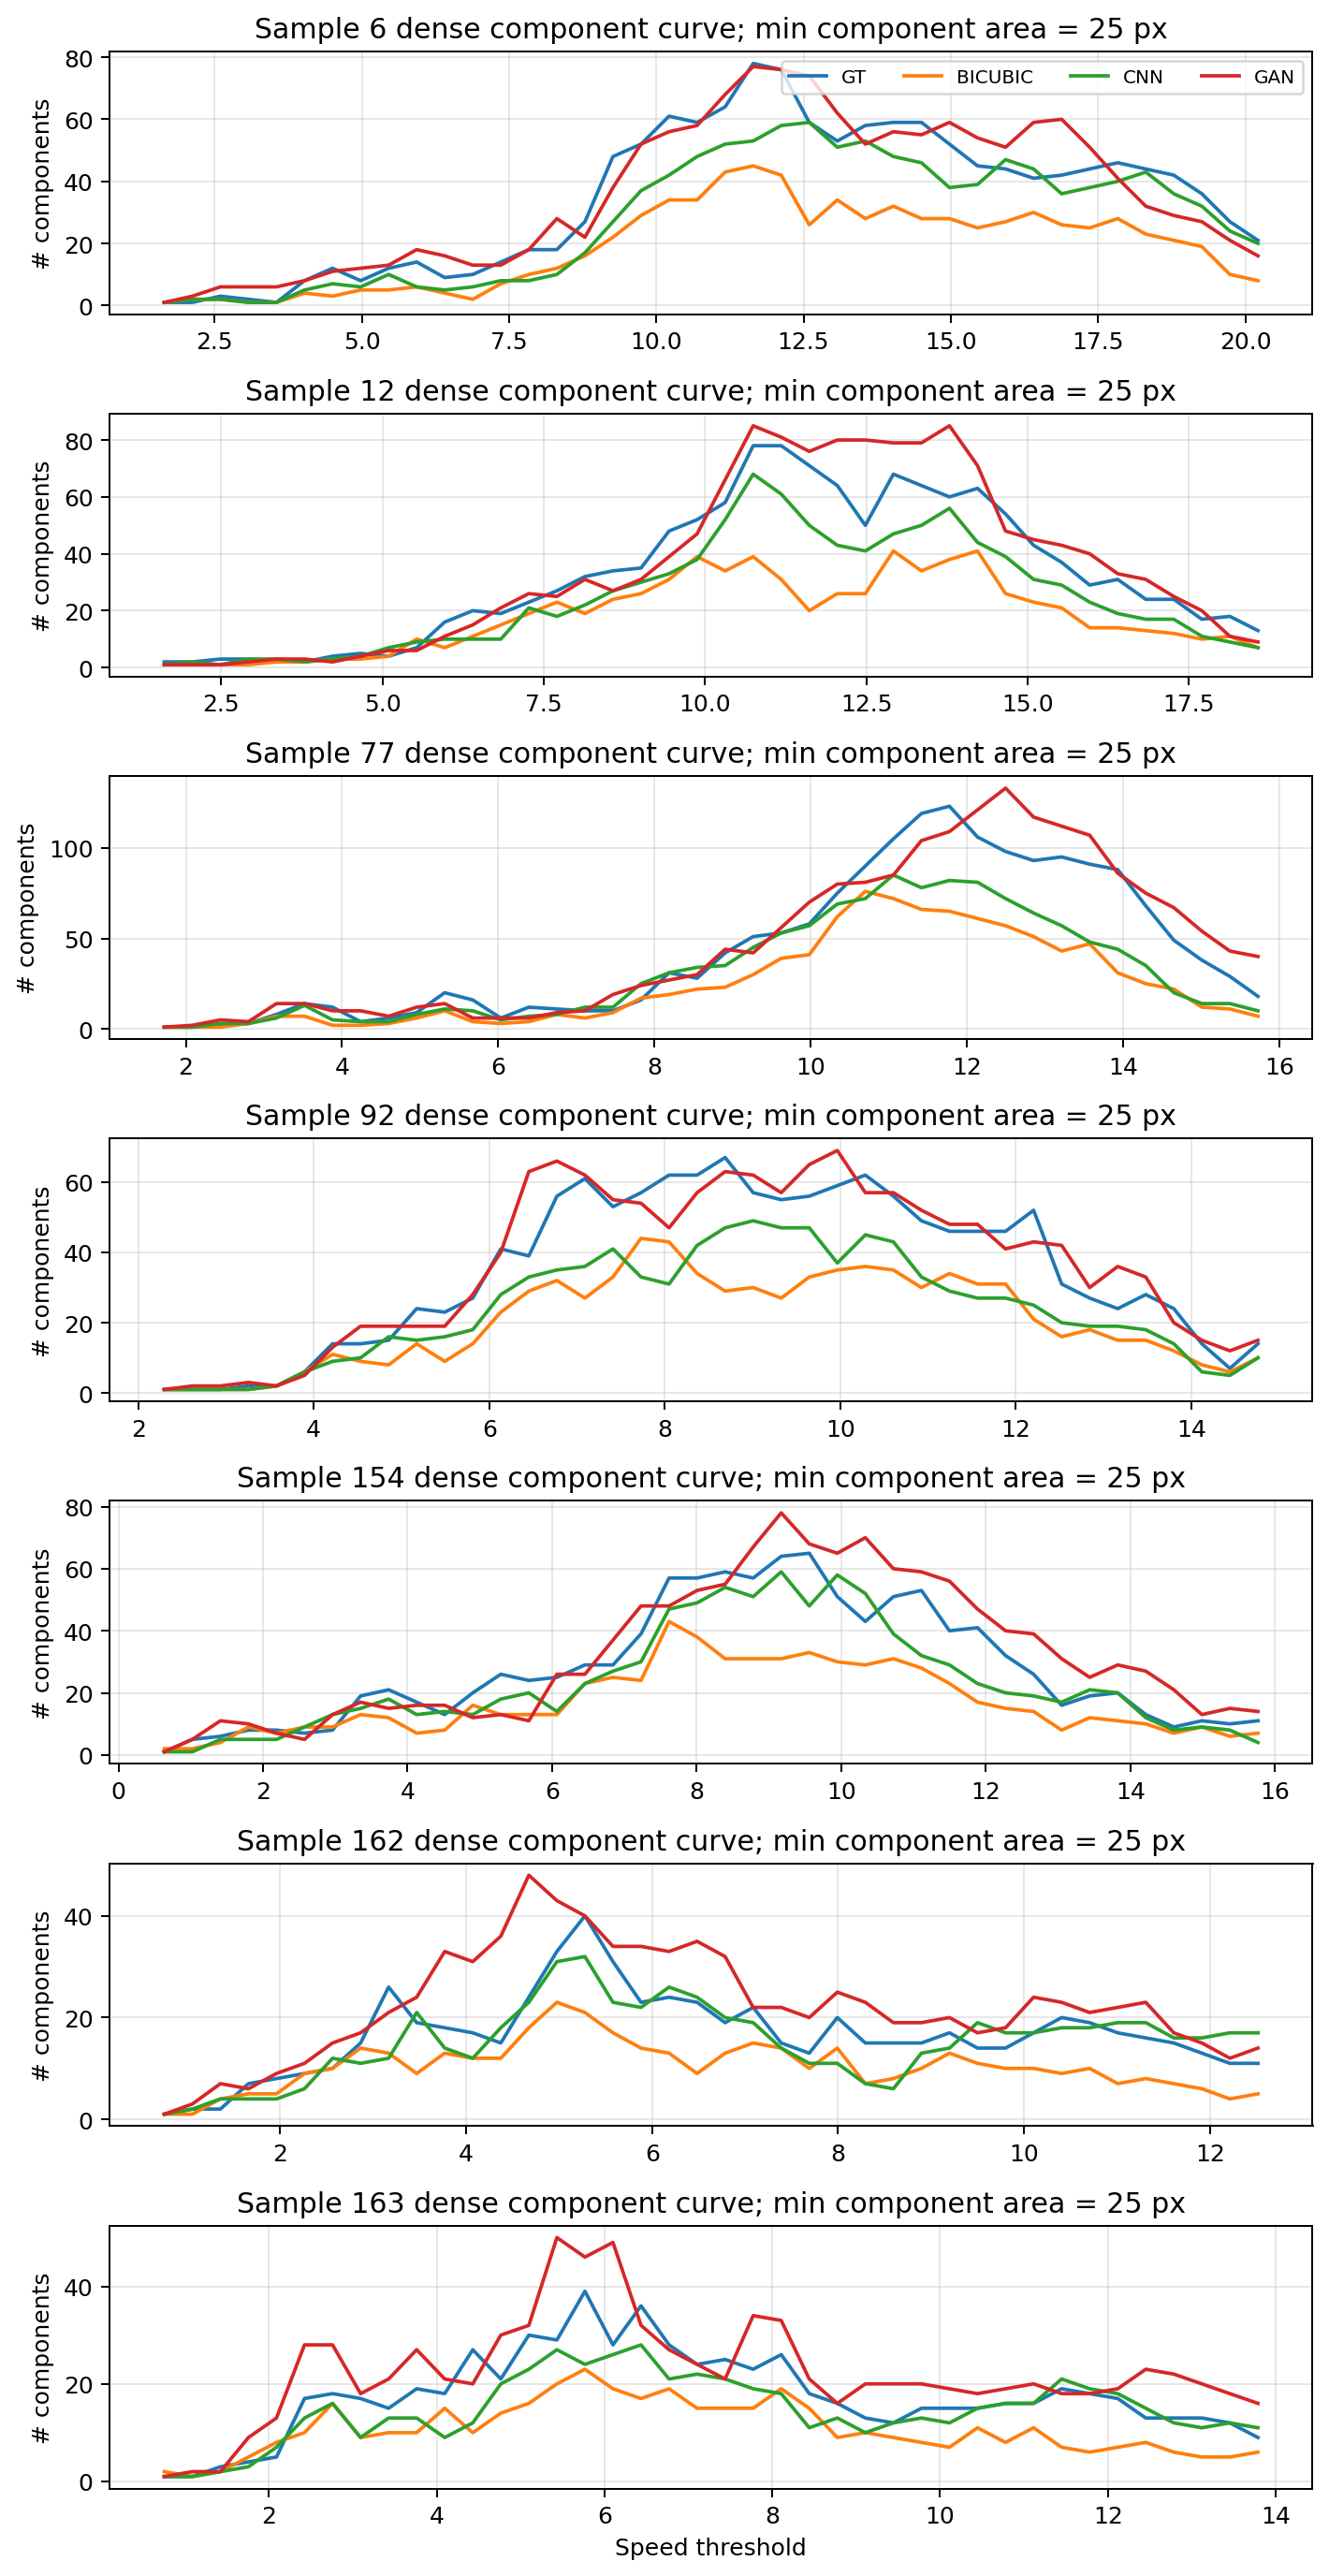
\includegraphics[width=0.92\textwidth]{figures/dense_component_curves.png}
    \caption{Dense component-count curves over many thresholds for representative samples. These curves are a richer component-based proxy than the six-threshold summary and help identify where GAN, CNN, or bicubic diverge from GT.}
    \label{fig:dense_component_curves_placeholder}
\end{figure*}

\subsection{Component-Lifetime Proxies}

A lightweight hierarchy proxy can be built by tracking connected components across adjacent thresholds. Even without full merge-tree matching, one can estimate approximate birth threshold, approximate death or merge threshold, component lifetime across threshold levels, number of long-lived components, total lifetime mass, and lifetime histogram distance to GT. These quantities are closer to merge-tree structure than single-threshold counts because they account for whether components persist across thresholds.

\subsection{Simplified-Tree Branch Counts}

A merge tree can be simplified by ignoring branches below a persistence threshold. For thresholds $\epsilon$, count the number of remaining branches:
\begin{equation}
    B_{\epsilon}(T) = \#\{\mathrm{branches\ in\ }T\mathrm{\ with\ persistence}>\epsilon\}.
\end{equation}
Comparing $B_{\epsilon}$ for GT, CNN, GAN, and bicubic across several $\epsilon$ values can test whether GAN's extra components correspond to meaningful branches or only low-persistence fragments.

\subsection{Branch Persistence Histograms}

For each merge tree, compute the distribution of branch persistence values. Useful summaries include number of branches above persistence thresholds, mean/median/maximum persistence, persistence histogram distance to GT, and cumulative persistence curves. This is easier than full tree visualization and can be compared across all 168 samples.

\subsection{Hierarchy Depth and Branching Statistics}

Additional tree-level summaries include number of leaves, number of internal merge nodes, maximum root-to-leaf depth, mean root-to-leaf depth, branching-factor distribution, size of largest subtree, and balance or imbalance of the tree. These are direct hierarchy proxies. If MT-GAN cases have tree-depth or branch-persistence summaries closer to GT than CNN, that would provide stronger evidence that MT is detecting meaningful hierarchy rather than merely counting components.

\begin{figure*}[t]
    \centering
    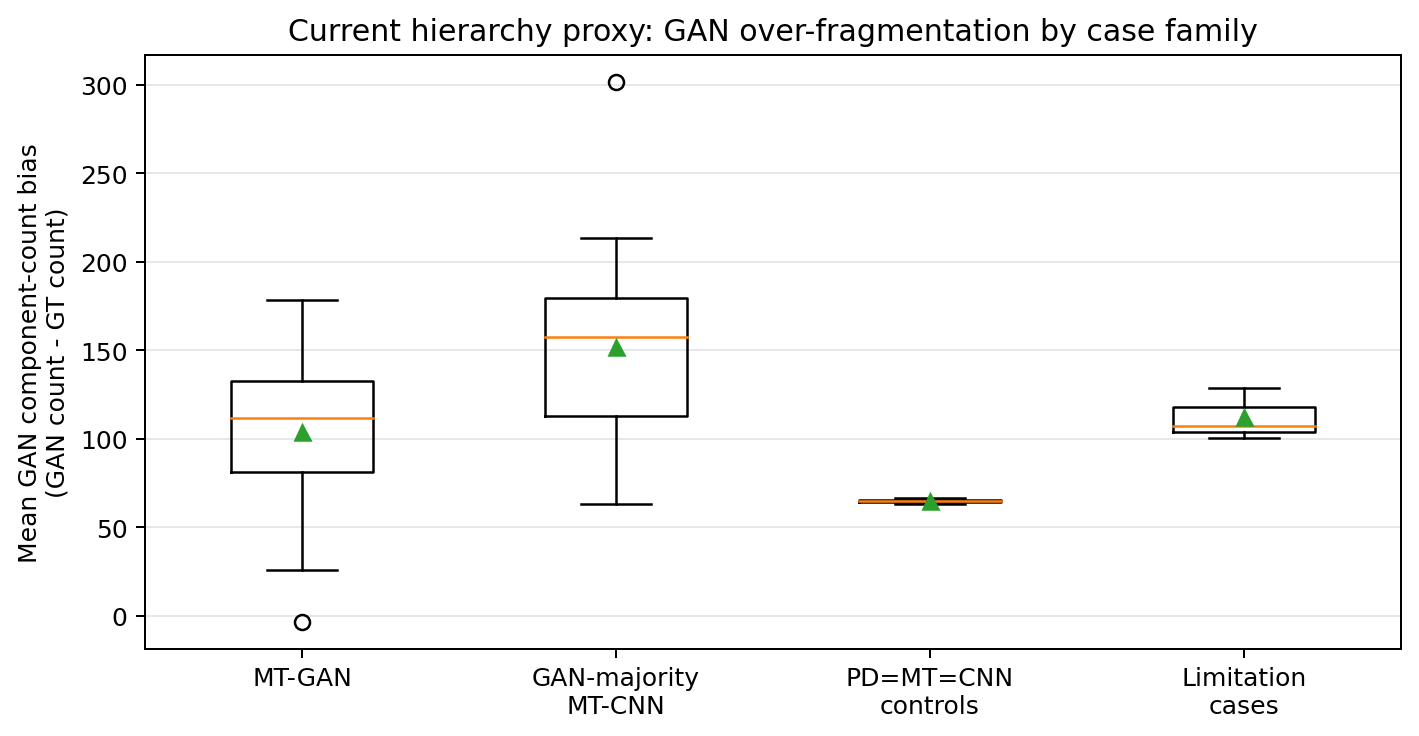
\includegraphics[width=0.48\textwidth]{figures/hierarchy_proxy_summary.png}
    \hfill
    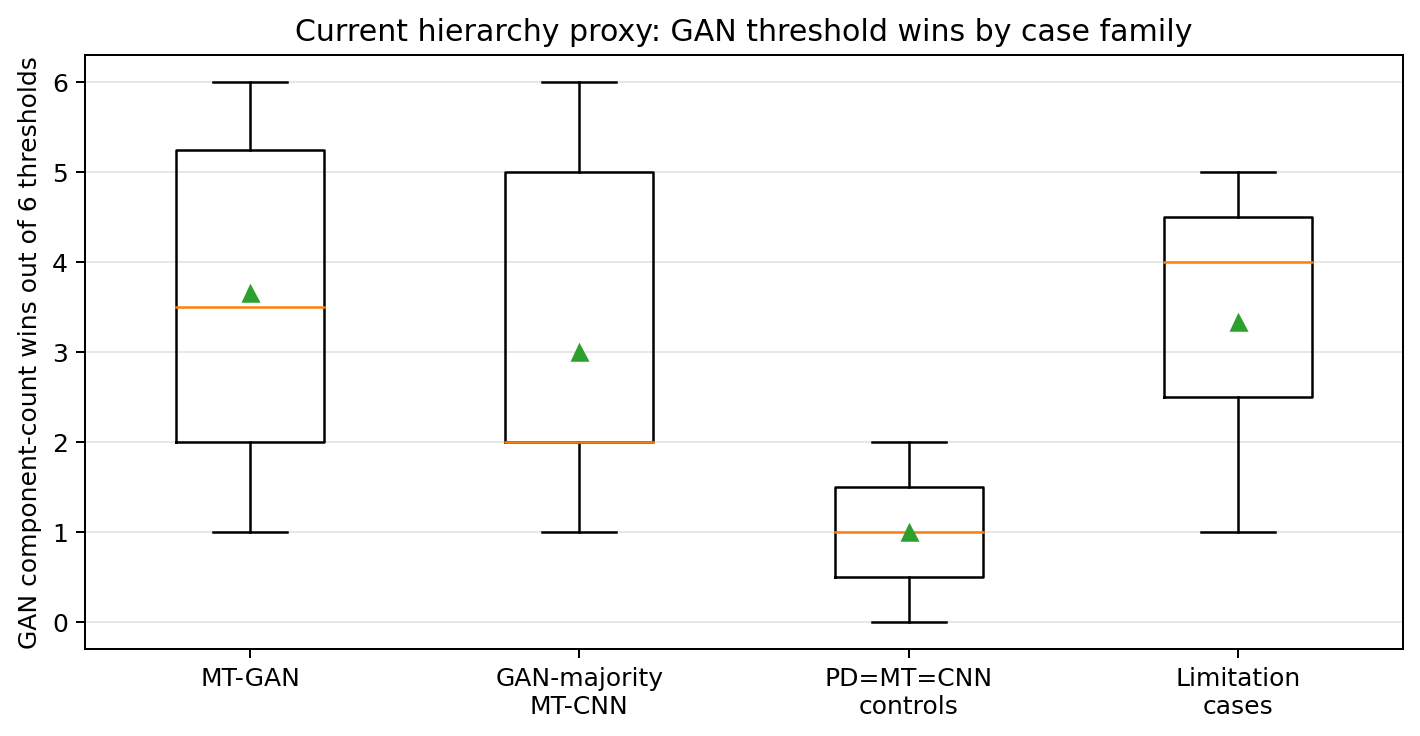
\includegraphics[width=0.48\textwidth]{figures/hierarchy_proxy_gan_wins.png}
    \caption{Current hierarchy proxies derived from component-count statistics. Left: GAN over-fragmentation bias by case family. Right: number of GAN component-count wins across six thresholds by case family. These are not full merge-tree summaries, but they provide a first bridge from raw component counts toward hierarchy-aware analysis.}
    \label{fig:hierarchy_proxy_summary}
\end{figure*}

% ============================================================
\section{Figure and Artifact Checklist}
% ============================================================

Table~\ref{tab:figure_checklist} lists the figures recommended for this report and where to obtain or generate them.

\begin{table*}[t]
\centering
\caption{Recommended report figures and where to obtain or create them.}
\label{tab:figure_checklist}
\begin{tabularx}{\textwidth}{p{0.18\textwidth}p{0.31\textwidth}p{0.43\textwidth}}
\toprule
Figure & Purpose & Source / generation path \\
\midrule
Pipeline schematic & Explain data, model, and evaluation flow & Draw manually from the current pipeline: NREL $\rightarrow$ MR/HR arrays $\rightarrow$ bicubic/CNN/GAN $\rightarrow$ metrics/topology/component counts. \\
Three-method metric summary & Show bicubic/CNN/GAN tradeoff & Use \texttt{ttk\_runs\_fixed/baseline\_metrics/all\_methods\_summary.csv} and \texttt{all\_methods\_winner\_counts.csv}. \\
Component threshold heatmap & Show threshold-dependent crossover & Use \texttt{ttk\_runs\_fixed/component\_counts/component\_count\_summary.csv} and \texttt{component\_count\_winner\_counts.csv}. \\
MT-GAN signature matrix & Classify the 20 MT-GAN cases & Use \texttt{ttk\_runs\_fixed/component\_counts/special\_component\_case\_summary.csv}, filter \texttt{group\_name=all\_mt\_gan}. \\
Adjacent cluster curves & Test local controls & Use \texttt{special\_component\_case\_thresholds.csv}, filter samples 10--13, 76--78, and 90--93. \\
Representative visual panels & Show GT/Bicubic/CNN/GAN and error maps & Use \texttt{ttk\_runs\_fixed/baseline\_visual\_panels/index.html} or PNGs in \texttt{panels\_crop/} and \texttt{panels\_full/}. \\
Rare topology-CNN controls & Show cases where both PD and MT reject GAN & Use samples 162 and 163 from \texttt{baseline\_visual\_panels/index.html}. \\
Hierarchy proxy summary & Move beyond component counts & Generate after extracting dense component curves, persistence histograms, branch counts, or simplified merge-tree summaries. \\
\bottomrule
\end{tabularx}
\end{table*}

% ============================================================
\section{Discussion}
% ============================================================

The component-count analysis adds a useful interpretive layer. Globally, bicubic and CNN under-represent component counts, while GAN restores component complexity at lower thresholds. However, GAN often over-fragments the high-speed tail. This supports a nuanced version of the earlier perception--distortion finding \cite{BlauMichaeli_2018}: smooth methods are accurate but structurally conservative, whereas GAN is structurally expressive but can create excessive high-threshold fragments.

The MT-GAN cases are not uniform. A small subset has strong component-count support for GAN across thresholds. Many others support GAN only at lower thresholds, suggesting that GAN may better match the broad structural skeleton while over-fragmenting high-speed details. Limitation cases such as sample 154 should be retained because they show that MT-GAN does not automatically imply broad metric support for GAN.

Most importantly, adjacent clusters show that component count alone cannot explain all MT decisions. In local temporal neighborhoods, adjacent samples can have similar component signatures while MT flips only for one sample. This suggests that MT may be sensitive to hierarchical information that is invisible to threshold-marginal component counts. That is precisely the reason to move toward branch-level and hierarchy-level diagnostics.

% ============================================================
\section{Implications for Topology-Aware Training}
% ============================================================

The current report motivates topology-aware scientific SR in two ways. First, the bicubic baseline shows that direct fidelity can be achieved without learned hallucination, but at the cost of reduced component complexity. Second, GAN shows that sharper outputs can restore component complexity, but may over-fragment high-speed regions. A useful topology-aware model should aim for the middle: retain bicubic/CNN-like point-wise and WPD accuracy while preserving meaningful multiscale structure.

A direct merge-tree distance loss may be difficult because exact MT distance is not naturally differentiable and can be expensive in a training loop. However, the present analysis suggests feasible surrogate losses:
\begin{itemize}
    \item dense soft component-count or level-set occupancy losses;
    \item losses on soft exceedance masks at physically meaningful thresholds;
    \item persistence-based losses on scalar wind speed \cite{KissiInterpolation_2025};
    \item branch-persistence or simplified-tree summary losses, if differentiable approximations are available;
    \item learned topological descriptor metrics, including merge-tree-related metric learning approaches \cite{QinDissertation_2025};
    \item hybrid losses combining pixel, WPD, PSD, gradient, and topology-inspired terms.
\end{itemize}

In the next experiment, exact PD and MT distances can remain post hoc evaluators, while trainable losses use differentiable proxies. The special cases identified here, especially samples 12, 77, 92, 162, 163, and 154, should be used as diagnostic examples for evaluating whether topology-aware training changes the structural behavior of the model.

% ============================================================
\section{Limitations}
% ============================================================

This report should be interpreted as an internal analysis and motivation document rather than a final model contribution. Current limitations include:
\begin{itemize}
    \item component counts are simple threshold-marginal summaries and do not encode merge hierarchy;
    \item raw component counts may be sensitive to small GAN speckles, so area-filtered variants should be tested;
    \item the results are based on one 168-sample evaluation slice;
    \item topology is computed on scalar speed magnitude, not on the full vector field;
    \item merge-tree branch-level interpretability has not yet been performed.
\end{itemize}

The next analysis should therefore compute dense component curves, area-filtered component counts, persistence/branch summaries, and simplified merge-tree statistics.

% ============================================================
\section{Conclusion}
% ============================================================

This report documents the component-count and special-case analysis stage of the wind-field SR topology project. The main finding is that component counts provide a useful but incomplete explanation for MT behavior. GAN often better matches GT component counts at lower thresholds, while CNN is more reliable at higher and percentile thresholds. Bicubic is strong under direct metrics but strongly under-counts components. The 20 MT-GAN cases split into strong, low-threshold-only, and limitation cases. Adjacent controls show that component count alone cannot explain every MT decision, suggesting that merge trees may capture additional hierarchy or nesting information. These results provide a concrete motivation for the next stage: extracting merge-tree-relevant hierarchy statistics and using them to design topology-aware SR training objectives.

\section*{Acknowledgments}

The author thanks Professor [Name], Qin [Last Name], and collaborators for feedback on the evaluation design, component-count analysis, and topology-aware training direction. [Add funding, lab, and compute acknowledgments here.]

\bibliographystyle{IEEEtran}
\bibliography{main}

\end{document}
